\documentclass[11pt]{article}
\usepackage[margin=1in]{geometry}
\usepackage{enumitem}
\usepackage{hyperref}
\usepackage{graphicx}
\usepackage{array}
\usepackage{multicol}
\usepackage{longtable}
\usepackage{titlesec}
\usepackage{float}
\usepackage{xcolor}
\usepackage{listings}

% Python code style
\lstdefinestyle{python}{
    language=Python,
    basicstyle=\ttfamily\footnotesize,
    keywordstyle=\color{blue},
    stringstyle=\color{red},
    commentstyle=\color{gray},
    showstringspaces=false,
    breaklines=true
}

\begin{document}

% ================= HEADER =================
\begin{center}
    \large \textbf{Sri Sivasubramaniya Nadar College of Engineering, Chennai} \\
    (An autonomous Institution affiliated to Anna University) \\
    \vspace{0.3cm}
\end{center}

\begin{table}[!h]
\renewcommand{\arraystretch}{1.5}
\resizebox{\textwidth}{!}{%
\begin{tabular}{|l|cll|}
\hline
Degree \& Branch     & \multicolumn{1}{c|}{B.E. Computer Science \& Engineering} & \multicolumn{1}{l|}{Semester}        & V                                        \\ \hline
Subject Code \& Name & \multicolumn{3}{c|}{ICS1512 \& Machine Learning Algorithms Laboratory} \\ \hline
Academic Year        & \multicolumn{1}{c|}{2025--2026 (Odd)} & \multicolumn{1}{c|}{Batch: 2023--2028} & \multicolumn{1}{c|}{\textbf{Due date: 25-07-25}} \\ \hline
\end{tabular}%
}
\end{table}

\begin{center}
 \LARGE \textbf{Experiment 2} \\
 \large Linear Regression for Loan Amount Prediction
\end{center}

% ================= AIM =================
\section*{Aim}
To apply Linear Regression for predicting the sanctioned loan amount using the given dataset. The model performance is assessed with cross-validation, error metrics, and visualization techniques.

% ================= LIBRARIES =================
\section*{Libraries Used}
\begin{itemize}
  \item pandas, numpy
  \item matplotlib, seaborn
  \item sklearn.linear\_model.LinearRegression
  \item sklearn.model\_selection.StratifiedKFold
  \item sklearn.metrics (MAE, MSE, RMSE, R\textsuperscript{2})
  \item sklearn.preprocessing (LabelEncoder, StandardScaler)
\end{itemize}

% ================= THEORY =================
\section*{Theoretical Description of the Algorithm}

\subsection*{Cross-Validation Strategy}
We employed a stratified 5-fold cross-validation setup. This ensured each fold retained a balanced target distribution, reducing bias and improving reliability of evaluation.

\subsection*{Data Preparation}
Irrelevant attributes (Customer ID, Property ID, Name) were dropped. Missing values were imputed (mean for numerical and mode for categorical), ensuring a clean dataset.

\subsection*{Feature Engineering}
Derived features included:
\begin{itemize}
    \item Loan-to-Income Ratio
    \item Total Expenses-to-Income Ratio
    \item Loan-to-Value (LTV) Category
\end{itemize}
These enhanced interpretability and credit risk analysis.

\subsection*{Encoding and Scaling}
Categorical features were label-encoded. Numerical features were standardized using \texttt{StandardScaler} for uniform scaling.

\subsection*{Model Training and Evaluation}
A Linear Regression model was trained and evaluated with error metrics (MAE, MSE, RMSE, \(R^2\), Adjusted \(R^2\)) and plots (Actual vs Predicted, Residuals, Feature Coefficients).

% ================= CODE =================

\section*{Complete Python Code}

\begin{lstlisting}[style=python]
# -*- coding: utf-8 -*-
"""ml_lab_2.ipynb

Automatically generated by Colab.

Original file is located at
    https://colab.research.google.com/drive/1hIn1DxB_VGEDuJ8OTAcpPE1Jldj33K9I
"""

from google.colab import files
import pandas as pd

# Upload the train dataset
uploaded = files.upload()

# Read the train dataset
df = pd.read_csv('train.csv')

# Check first few rows
df.head()

# Check missing values
print("Before filling missing values:")
print(df.isnull().sum())

# Fill missing numerical values with mean
numeric_cols = df.select_dtypes(include=['float64', 'int64']).columns
for col in numeric_cols:
    df[col] = df[col].fillna(df[col].mean())

# Fill missing categorical values with mode
categorical_cols = df.select_dtypes(include=['object']).columns
for col in categorical_cols:
    if df[col].isnull().any():
        df[col] = df[col].fillna(df[col].mode()[0])

# Verify no missing values remain
print("\nAfter filling missing values:")
print(df.isnull().sum())

# Display first few rows to check
df.head()

"""feature engineering"""

unnecessary_columns = ['Customer ID', 'Name', 'Property ID']
df.drop(columns=unnecessary_columns, inplace=True)

# Convert required columns to numeric
df['Loan Amount Request (USD)'] = pd.to_numeric(df['Loan Amount Request (USD)'], errors='coerce')
df['Property Price'] = pd.to_numeric(df['Property Price'], errors='coerce')
df['Income (USD)'] = pd.to_numeric(df['Income (USD)'], errors='coerce')
df['Current Loan Expenses (USD)'] = pd.to_numeric(df['Current Loan Expenses (USD)'], errors='coerce')

# 1. LTV Risk Category
def ltv_risk_category(row):
    loan_amount = row['Loan Amount Request (USD)']
    property_price = row['Property Price']
    if pd.isna(loan_amount) or pd.isna(property_price) or property_price == 0:
        return 'Unknown'
    ltv = loan_amount / property_price
    if ltv >= 0.9:
        return 'Very High'
    elif ltv >= 0.75:
        return 'High'
    elif ltv >= 0.6:
        return 'Moderate'
    else:
        return 'Low'

df['LTV_Risk'] = df.apply(ltv_risk_category, axis=1)

# 2. Loan-to-Income Ratio
df['Loan_to_Income'] = df['Loan Amount Request (USD)'] / (df['Income (USD)'] + 1e-5)

# 3. Total Expenses-to-Income Ratio
df['Total_Expenses_to_Income'] = df['Current Loan Expenses (USD)'] / (df['Income (USD)'] + 1e-5)

# Preview dataset
df.head()

from sklearn.preprocessing import LabelEncoder
label_encoders = {}
for col in df.select_dtypes(include=['object']).columns:
    df[col] = df[col].astype(str)
    le = LabelEncoder()
    df[col] = le.fit_transform(df[col])
    label_encoders[col] = le

df.head()

from sklearn.preprocessing import StandardScaler
scaler = StandardScaler()
features = df.drop('Loan Sanction Amount (USD)', axis=1)
fs = scaler.fit_transform(features)
fs = pd.DataFrame(fs, columns=features.columns)
fs['Loan Sanction Amount (USD)'] = df['Loan Sanction Amount (USD)']
fs.head()

"""EDA"""

print("Dataset shape:", fs.shape)
print("\nData types:\n", fs.dtypes)
fs.head()
fs.describe()

"""Visualizations"""

import matplotlib.pyplot as plt
import seaborn as sns

plt.figure(figsize=(8,5))
sns.histplot(fs['Loan Sanction Amount (USD)'], kde=True, bins=30)
plt.title('Distribution of Loan Sanction Amount (USD)')
plt.show()

plt.figure(figsize=(15,10))
for i, col in enumerate(fs.columns.drop('Loan Sanction Amount (USD)'), 1):
    plt.subplot(5, 5, i)
    sns.histplot(fs[col], kde=True)
    plt.title(col)
    plt.tight_layout()
plt.show()

plt.figure(figsize=(12,10))
corr = fs.corr()
sns.heatmap(corr, annot=True, cmap='coolwarm', fmt=".2f")
plt.title('Correlation Matrix of Scaled Features and Target')
plt.show()

"""Model Training and Cross-Validation"""

import numpy as np
from sklearn.model_selection import StratifiedKFold
from sklearn.linear_model import LinearRegression
from sklearn.metrics import mean_absolute_error, mean_squared_error, r2_score

X = fs.drop('Loan Sanction Amount (USD)', axis=1)
y = fs['Loan Sanction Amount (USD)']
X = pd.get_dummies(X, drop_first=True)
y_binned = pd.qcut(y, q=5, labels=False, duplicates='drop')

skf = StratifiedKFold(n_splits=5, shuffle=True, random_state=42)
mae_scores, mse_scores, rmse_scores, r2_scores, adj_r2_scores = [], [], [], [], []
results, fold = [], 1

def adjusted_r2(r2, n, k):
    return 1 - (1 - r2) * (n - 1) / (n - k - 1)

saved = False
for train_idx, val_idx in skf.split(X, y_binned):
    X_train_fold, X_val_fold = X.iloc[train_idx], X.iloc[val_idx]
    y_train_fold, y_val_fold = y.iloc[train_idx], y.iloc[val_idx]

    if not saved:
        X_train, y_train, X_val, y_val = X_train_fold, y_train_fold, X_val_fold, y_val_fold
        saved = True

    model = LinearRegression()
    model.fit(X_train_fold, y_train_fold)
    y_pred = model.predict(X_val_fold)

    mae = mean_absolute_error(y_val_fold, y_pred)
    mse = mean_squared_error(y_val_fold, y_pred)
    rmse = np.sqrt(mse)
    r2 = r2_score(y_val_fold, y_pred)
    adj_r2 = adjusted_r2(r2, X_val_fold.shape[0], X_val_fold.shape[1])

    mae_scores.append(mae); mse_scores.append(mse); rmse_scores.append(rmse)
    r2_scores.append(r2); adj_r2_scores.append(adj_r2)
    results.append([f"Fold {fold}", mae, mse, rmse, r2, adj_r2])
    fold += 1

results.append(["Average", np.mean(mae_scores), np.mean(mse_scores),
                np.mean(rmse_scores), np.mean(r2_scores), np.mean(adj_r2_scores)])

cv_results_df = pd.DataFrame(results, columns=["Fold","MAE","MSE","RMSE","R²","Adj R²"])
print(cv_results_df)

"""Plots"""

plt.figure(figsize=(8,6))
sns.scatterplot(x=y_val, y=model.predict(X_val))
plt.xlabel("Actual Loan Amount")
plt.ylabel("Predicted Loan Amount")
plt.title("Actual vs Predicted Loan Amount")
plt.plot([y_val.min(), y_val.max()], [y_val.min(), y_val.max()], color='red', linestyle='--')
plt.grid(True)
plt.tight_layout()
plt.show()

residuals = y_val - model.predict(X_val)
plt.figure(figsize=(8,6))
sns.scatterplot(x=model.predict(X_val), y=residuals)
plt.axhline(0, color='red', linestyle='--')
plt.xlabel("Predicted Loan Amount")
plt.ylabel("Residuals")
plt.title("Residual Plot")
plt.grid(True)
plt.tight_layout()
plt.show()

numerical_cols = ['Income (USD)','Loan Amount Request (USD)','Age','Current Loan Expenses (USD)']
plt.figure(figsize=(14,8))
for i, col in enumerate(numerical_cols, 1):
    plt.subplot(2, 2, i)
    sns.boxplot(y=fs[col])
    plt.title(f'Boxplot of {col}')
    plt.tight_layout()
plt.show()

model = LinearRegression()
model.fit(X_train, y_train)
coefficients = pd.Series(model.coef_, index=X_train.columns)

plt.figure(figsize=(10,6))
coefficients.sort_values().plot(kind='barh', color='skyblue')
plt.title('Feature Coefficients from Linear Regression')
plt.xlabel('Coefficient Value')
plt.ylabel('Features')
plt.grid(True)
plt.tight_layout()
plt.show()
\end{lstlisting}


% ================= OUTPUT =================
\section*{Screenshots of Output}
\begin{figure}[H]
    \centering
    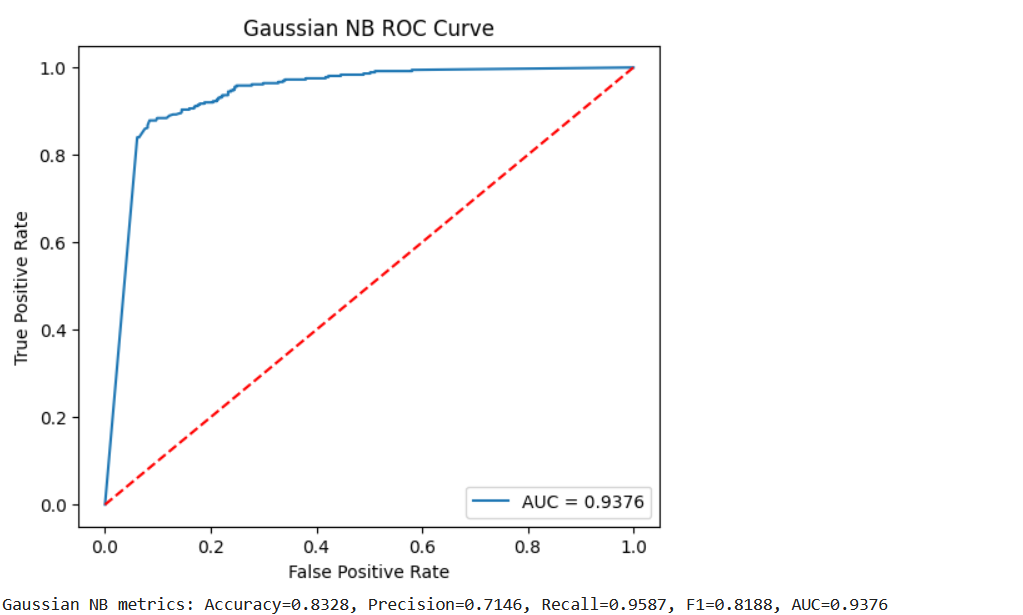
\includegraphics[width=0.8\textwidth]{7}
    \caption{Feature Distribution Visualization}
\end{figure}

\begin{figure}[H]
    \centering
    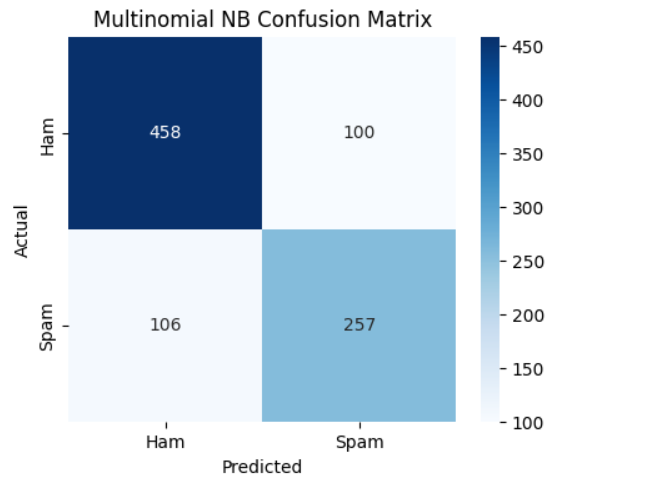
\includegraphics[width=0.8\textwidth]{8}
    \caption{Correlation Heatmap}
\end{figure}

\begin{figure}[H]
    \centering
    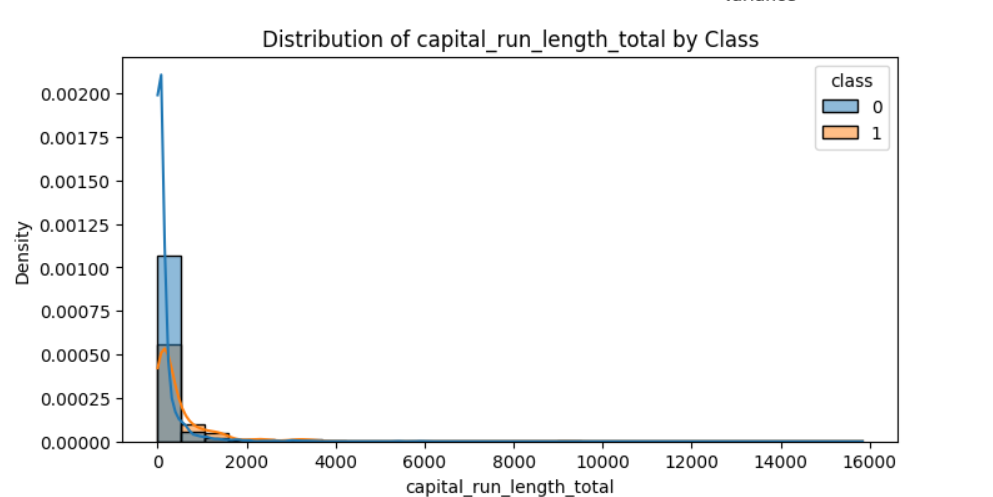
\includegraphics[width=0.8\textwidth]{3.png}
    \caption{Actual vs Predicted Loan Amount}
\end{figure}

\begin{figure}[H]
    \centering
    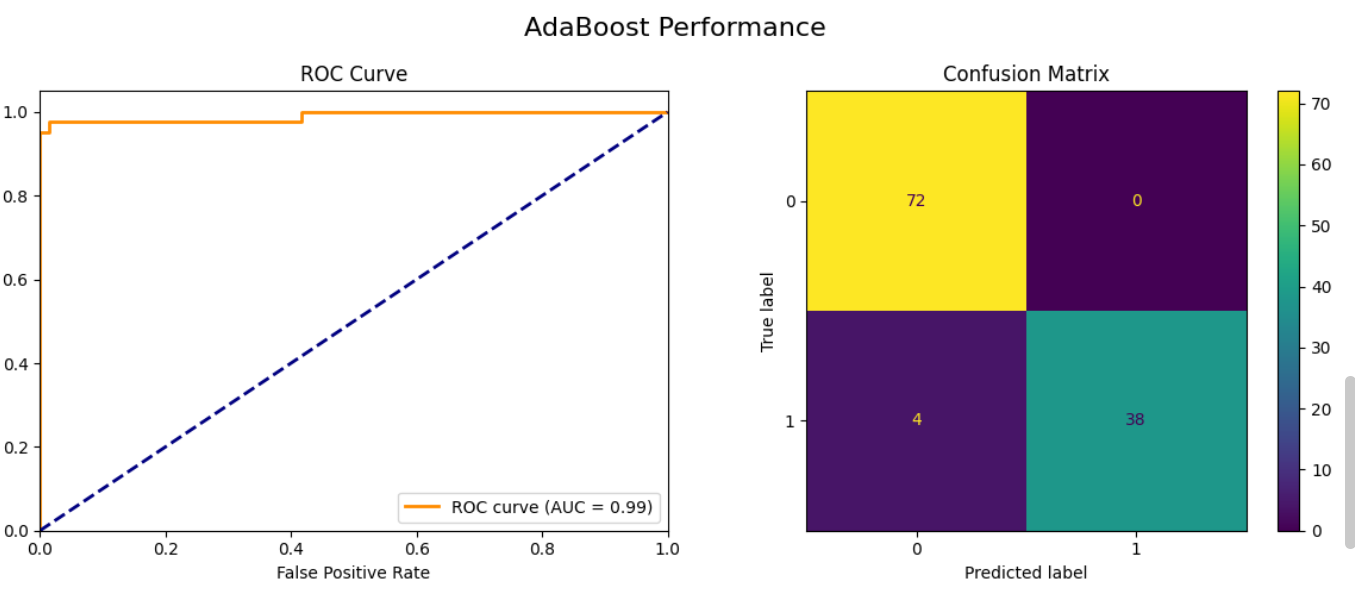
\includegraphics[width=0.8\textwidth]{4.png}
    \caption{Residual Plot}
\end{figure}

% ================= RESULTS =================
\section*{Results and Discussions}

\subsection*{Cross-Validation Metrics}
\begin{table}[h!]
\centering
\begin{tabular}{|c|c|c|c|c|c|}
\hline
Fold & MAE & MSE & RMSE & R\textsuperscript{2} Score & Adj. R\textsuperscript{2} Score \\ \hline
1 & 21855.65 & $9.77 \times 10^8$ & 31254.23 & 0.5738 & 0.5722 \\
2 & 21883.08 & $9.78 \times 10^8$ & 31275.97 & 0.5830 & 0.5814 \\
3 & 21608.39 & $9.60 \times 10^8$ & 30987.54 & 0.5681 & 0.5664 \\
4 & 21668.17 & $9.67 \times 10^8$ & 31094.08 & 0.5834 & 0.5818 \\
5 & 21957.28 & $1.19 \times 10^9$ & 34491.73 & 0.4855 & 0.4835 \\ \hline
\textbf{Average} & \textbf{21794.51} & \textbf{$1.01 \times 10^9$} & \textbf{31820.71} & \textbf{0.5588} & \textbf{0.5571} \\ \hline
\end{tabular}
\caption{Cross-validation results with Adjusted R\textsuperscript{2}}
\end{table}

\subsection*{Summary of Results}
\begin{table}[H]
\centering
\begin{tabular}{|p{8cm}|p{6cm}|}
\hline
\textbf{Description} & \textbf{Student’s Result} \\ \hline
Dataset Size & 50,000 rows × 25 columns \\ \hline
CV Strategy & 5-Fold Stratified \\ \hline
Model Used & Linear Regression \\ \hline
Avg. MAE & 21,794.51 USD \\ \hline
Avg. RMSE & 31,820.71 USD \\ \hline
R\textsuperscript{2} & 0.5588 \\ \hline
Adj. R\textsuperscript{2} & 0.5571 \\ \hline
Most Influential Features & Loan Amount Request, Income, Loan-to-Income Ratio \\ \hline
Observations & Underestimation for very high loan amounts; mild underfitting \\ \hline
\end{tabular}
\caption{Summary of Loan Prediction Results}
\end{table}

% ================= PERFORMANCE =================
\subsection*{Performance Analysis}
\begin{itemize}
    \item Average MAE $\approx$ 21,795 USD shows the typical deviation from actual loans.
    \item RMSE of 31,821 USD indicates slightly higher penalty for large errors.
    \item \(R^2 = 0.56\) shows moderate explanatory power (56\% variance explained).
    \item Adjusted \(R^2\) nearly equal, meaning predictors are not excessive.
    \item Residual plot shows mild underfitting, especially for extreme values.
\end{itemize}

% ================= LEARNING =================
\section*{Learning Outcomes}
\begin{itemize}
    \item Applied Linear Regression to a financial dataset.
    \item Learned stratified cross-validation for regression tasks.
    \item Practiced preprocessing: missing value handling, encoding, scaling.
    \item Understood evaluation metrics for regression (MAE, MSE, RMSE, \(R^2\)).
    \item Interpreted residuals and coefficients for model insights.
\end{itemize}

\end{document}
